%\chapter*{История ОНТИ}

\begingroup
\pagestyle{empty}
\section*{Введение}

Задачи профиля связаны с актуальными задачами систем связи, включая вопросы помехоустойчивого кодирования, передачи информации в условиях шумов, работы с различными форматами данных, разработки адаптивной системы слежения и т.д. Ключевые области применения связаны с Космосом, промышленным интернетом вещей, подводной и мобильной робототехникой, каналами связи для роевых устройств.

В ходе решения заданий командного тура заключительного этапа командам предстояло решать задачи, связанные с помехоустойчивым кодированием и декодированием, передачей данных по каналам с различной зашумленностью и скоростью, алгоритмами слежения за объектом с частично детерминированной траекторией. Для этого участникам необходимо было разобраться с физическими свойствами закодированного сигнала, программными алгоритмами разбиения данных на блоки с различной избыточностью кодирования для различных каналов, а также с восстановлением по данным физического моделирования траекторной информации и диаграммы направленности.  

Задачи были составлены таким образом, что для их решения требуются знания не только школьного уровня, но и углубленные знания в области по программирования, математики и геометрии, а также азы по помехоустойчивому кодированию. От этапа к этапу увеличивалась, как сложность задач, так и их специфика. По мере продвижения команд к финальному испытанию проводились хакатоны, предоставлялись дополнительные методические материалы по сложным темам: методы исследования каналов связи и обработки сигналов, методы борьбы с шумами, получение практических навыков по помехоустойчивому кодированию в системах связи, практика работы с бинарными файлами - байтами и битами, практика работы с анализом информации разных типов: графической, текстовой.

Первый отборочный этап определял общий уровень подготовки школьников по предметам математика и информатика. Решая задачи по программированию, школьники должны были продемонстрировать простейшие навыки составления и отладки программ, обрабатывающих массивы данных, и понимание таких тем, как битовые операции, строковые операции, теория графов. Успешное решение данных задач доказывало готовность участников к работе с обучающими материалами второго этапа. Задачи по математике проверяли у участников углубленные знания некоторых тем из школьной программы.

Задачи второго этапа сформулированы таким образом, чтобы отразить специфику профиля, они более сложные и затрагивают актуальные темы в системах связи, а также готовят команды к задачам финального испытания. Кроме того, задачи второго этапа направлены на развитие  элементов научного исследовательского подхода и навыков командной работы. Для решения задач второго этапа достаточно школьных знаний и умений программы 10-11 класса, а также навыков использовать школьные знания для решения новых задач. Во втором этапе было 5 задач, цель которых - как отбор, так и подготовка командному туру заключительного этапа.  Данный этап задает область предметных знаний необходимую для участия в профиле. Методические рекомендации к данному этапу позволяют очертить область знаний и навыков для самостоятельного изучения. Все задачи этапа сочетают в себе математику и информатику. 

На заключительном этапе в командном туре каждая команда профиля «Технологии беспроводной связи» работала с экспериментальным стендом, разработанным специально для проведения заключительного этапа данного профиля, более подробное описание стенда приведено в приложении к материалам заданий профиля.

По условию финальной задачи удаленный объект передает данные телеметрии, на основании которых необходимо определить техническое состояние объекта, и если объект неисправен, то определить характер неисправности. В распоряжении команд имеется эталонная модель спутника, с помощью которой можно получить корректную телеметрию (т.е. такую, которую передает полностью исправный спутник) и на основе сравнительного анализа определить причину сбоя, результаты исследования занести в диагностическую карту.

Необходимо, используя предложенные беспроводные каналы связи, организовать устойчивый канал передачи телеметрии, локализовать возникшие ошибки на спутнике и расширить его функциональные возможности, задействовав дополнительный технологический канал. Подобная задача регулярно возникает при восстановлении работоспособности автоматических космических аппаратов или других удаленных объектах, работающих в неблагоприятных условиях.

Задачи финального испытания составлены таким образом, чтобы они образовывали взаимосвязанную цепочку. Все задачи заключительного этапа были связаны с задачами первого и второго этапов. Также в заключительный этап входил индивидуальный предметный тур, в ходе которого участники решали задачи по математике и информатике. Ниже приведены таблицы взаимосвязи финальных задач с задачами второго этапа и задачами индивидуального тура финала с перечислениями навыков и знаний, которые нужны школьникам для решения. 
\begin{center}
\small
\begin{longtable}{|p{2cm}|p{11cm}|p{2cm}|}
\hline
\textbf{№ задачи 2-го этапа} & \textbf{ Знания и навыки, на выявление и развитие которых
направлена задача} & \textbf{№ задачи в командном туре финала} \\
\hline
1. Чет-нечет & Нацелена на развитие: алгоритмического мышления, знакомству с базовым алгоритмом помехоустойчивого кодирования (кодом Хэмминга).

Для решения задачи необходимы разделы информатики, посвященные следующим темам:
обработка простых массивов данных, выявление периодичностей в данных, работа с чтением/записью файлов.

Для решения задачи необходимы разделы математики, посвященные следующим темам: теория вероятности алгебраический анализ данных.
& 1,2 \\
\hline
2. Веселый спутник & Нацелена на выявление и развитие алгоритмического мышления, умение работать с различными системами координат, понимание принципов корреляционной обработки данных.

Для решения задачи необходимы разделы информатики, посвященные следующим темам: работа с массивами, работа с циклами, чтение и запись файлов.

Для решения задачи необходимы разделы математики, посвященные следующим темам: работа с системами координат: декартова, сферическая, представления в них данных, корреляционный анализ. & 3, 4, 5 \\
\hline
3. Космический вальс & Нацелена на развитие навыков математического моделирования, аппроксимации функций и решению обратных задач.

Требует в основном факультативных знаний, доступных школьнику. Материалы по данным разделам представлены в методических материалах к профилю.

Для решения задачи необходимы разделы информатики, посвященные следующим темам: способность работать с рядами данных, использование рекурсивных алгоритмов, работа с организацией стека памяти, чтение и запись файлов.

Для решения задачи необходимы разделы математики, посвященные следующим темам: алгебраическая запись декартовой метрики для плоскости, применение аффинных преобразований: поворот, отражение, трансляция, работа с тригонометрическими функциями. & 3, 4, 5 \\
\hline
4. Два канала & Нацелена на развитие навыков работы с теорией вероятности, на понимание таких важных понятий как отношение сигнала/шум, условная вероятность, независимые и зависимые события.

Требует в основном факультативных знаний, доступных школьнику. Материалы по данным разделам представлены в методических материалах к профилю.

Для решения задачи необходимы разделы информатики, посвященные следующим темам: методы численного корреляционного анализа.

Для решения задачи необходимы разделы математики, посвященные следующим темам: теория информации, теория вероятности. & 1, 2 \\
\hline
5. Сложный рельеф & Нацелена на развитие навыков работы с анализом большого объема данных в условиях серьезных ограничений, как по времени обработки, так и по объему используемой памяти. Развитию навыков применения знаний по геометрии. 

Требует в основном факультативных знаний, доступных школьнику. Материалы по данным разделам представлены в методических материалах к профилю.

Для решения задачи необходимы разделы информатики, посвященные следующим темам: работа с массивами, работа с циклами, разработка оптимальных алгоритмов,  чтение и запись файлов.

Для решения задачи необходимы разделы математики, посвященные следующим темам: работа с тригонометрическими функциями, базовые знания их планиметрии, алгебраическая запись декартовой метрики для плоскости. & 5 \\
\hline
\end{longtable}
\end{center}

\textbf{Заключительный этап: индивидуальная часть}

\textbf{Задачи предметного тура по математике}

В таблице приведены номера задач предметного индивидуального тура, элементы решения которых или, полученное в результате решения, понимание могут быть использованы для решения задач командного тура в финале. Такое соотнесение навыков позволяет лучше учесть личный вклад в командный результат.

\begin{center}
\small
\begin{longtable}{|p{2cm}|p{7cm}|p{6cm}|}
\hline
\textbf{№ задач} & \textbf{ Знания и навыки, на выявление и развитие которых направлена задача} & \textbf{№ задачи на командном туре в финале, в которой применимо} \\
\hline
1& Решение задачи требует навыков работы с множественными условиями и системами уравнений.& Задача 1. Поиск периодичности в данных.

Задача 4. Определение параметров траектории. \\
\hline
2 & Решение задачи требует владения элементарной теорией вероятностей. & Задача 2. Анализ шумов и помех в канале передачи данных. \\
\hline
3 & Для решения задачи нужно владение элементарной теорией вероятностей, навыки комбинаторики и пространственного мышления.& Задача 2. Анализ шумов и помех в канале передачи данных.

Задача 5. Поиск объектов определенного/ заданного типа, по некоторому пороговому статистически значимому уровню.\\
\hline
4& Для решения задачи нужно владение элементарной теорией вероятностей и техниками работы с бесконечными системами.& Задача 2.\\
\hline
5& Решение задачи требует владения алгебраической геометрией и планиметрией.& Задачи 3, 4.\\
\hline
5& Решение задачи требует владения алгебраической геометрией и планиметрией.& Задачи 3, 4.\\
\hline
\end{longtable}
\end{center}

\textbf{Задачи предметного тура по информатике}

В таблице приведены номера задач предметного индивидуального тура, элементы решения которых или, полученное в результате решения, понимание могут быть использованы для решения задач командного тура в финале. Такое соотнесение навыков позволяет лучше учесть личный вклад в командный результат.

\begin{center}
\small
\begin{longtable}{|p{2cm}|p{9cm}|p{4cm}|}
\hline
\textbf{№ задач} & \textbf{Знания и навыки, на выявление и развитие которых направлена задача}&\textbf{№ задачи на командном туре в финале, в которой применимо} \\
\hline
1 & Для решения задачи необходимы разделы информатики и математики, посвященные следующим темам: системы счисления, десятичные дроби, рациональные и иррациональные числа.& Задача 1. Поиск периодичности в данных, работа в разных системах счисления.\\
\hline
2& Для решения задачи необходимы разделы математики и информатики, посвященные следующим темам: решение задач типа «рюкзак», теория вероятностей.& Задача 2.

Задача 3.\\
\hline
3& Для решения задачи необходимы разделы математики и информатики, посвященные следующим темам: теория вероятностей, полный перебор, работа чтением данных из числовых массивов. & Задача 1.

Задача 2.\\
\hline
4& Для решения задачи необходимы разделы математики и информатики, посвященные следующим темам: циклы, условные операторы, работа с двумерными массивами.& Задача 3.

Задача 5. Использование оптимальных алгоритмов перебора(обхода) данных \\
\hline
5& Для решения задачи необходимы разделы математики и информатики, посвященные следующим темам: графы, свёртка дерева.& Задача 4.

Задача 5. \\
\hline
\end{longtable}
\end{center}

\textbf{Заключительный этап: командный тур}

Задачи командного тура профиля заключительного этапа составлены таким образом, чтобы они, с одной стороны, были достаточно независимыми, а с другой образовывали взаимосвязанную цепочку, необходимую для решения финальной задачи. Количество одновременно решаемых задач определяет слаженность командной работы. Всего командам предлагается 5 задач, в каждой команде по 3 -5 человек, таким образом, каждый участник может решать свою задачу. 

Краткое описание командных задач финала:
\begin{enumerate}
\item Работа с узором шестеренки - определение кода Хемминга и декодирование. Определение закодированного десятичного числа. Определение среднего периода обращения и среднеквадратичного отклонения от среднего периода – результаты вносятся в диагностическую карту.
\item Передача данных со спутника (кодирование/декодирование, сжатие, разбиение на блоки). Тестирование программ кодера и декодера в модельных каналах с различным уровнем сложности распределения ошибок.
\item Разработка алгоритма слежения за спутником.
\item Анализ телеметрической информации, полученной по техническому каналу.  Анализ телеметрии, определение параметров траектории: большая и малая полуоси орбиты естественного спутника, период обращения естественного спутника вокруг планеты, радиус круговой орбиты и период обращения искусственного спутника вокруг естественного спутника. Результаты анализа заносятся в диагностическую карту.
\item Разработка алгоритма и программы определения положений и размеров кратеров на большой карте, содержащей также различные «помеховые» элементы рельефа.
\end{enumerate}

На представленном ниже рисунке, представлено дерево задач с разбивкой на подзадачи.

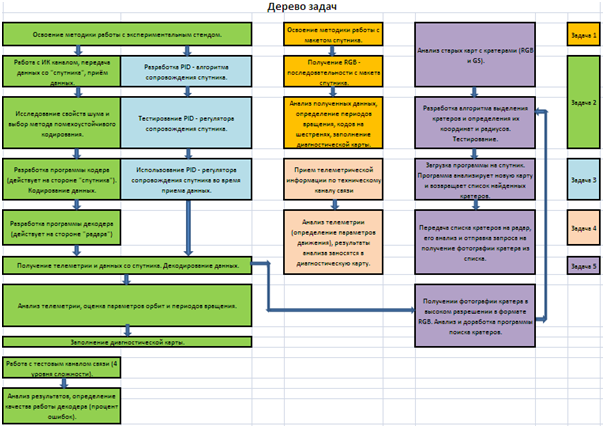
\includegraphics[width=15cm]{history/telecom/telecom.png}

%\begin{center} Дерево задач профиля ТБС \end{center}

При решении задач в основном требуются факультативные знания, доступные школьнику. Материалы по данным разделам представлены в методических материалах к профилю.

\begin{center}
\small
\begin{longtable}{|p{2cm}|p{10cm}|p{3cm}|}
\hline
\textbf{№ задач}&\textbf{Знания и навыки, на выявление и развитие которых направлена задача}& \textbf{Связь между задачами в командном туре} \\
\hline
1& Для решения задачи необходимы разделы информатики, посвященные темам: работа с помехоустойчивым кодом Хемминга, исправляющим однократную ошибку, алгоритмы кодирования и декодирования сообщения. 

Для решения задачи необходимы разделы математики, посвященные темам: периодические функции, работа со статистическим анализом данных - определение среднего и среднеквадратичного отклонения.& Результаты решения задачи могут быть использованы при решении задач 2 и 5. \\
\hline
2& Для решения задачи необходимы разделы информатики, посвященные темам: работа с помехоустойчивым кодированием, алгоритмы кодирования и декодирования сообщения, работа с байтами и битами (с бинарными файлами), работа с пакетной передачей данных. 

Для решения задачи необходимы разделы математики, посвященные темам: работа со статистическим анализом данных.& Результаты решения задачи могут быть использованы при решении задачи 5. \\
\hline
3& Для решения задачи необходимы разделы информатики, посвященные следующим темам: работа по проектированию предсказательных алгоритмов, в частности алгоритмов сопровождения движущихся объектов, работа с программным интерфейсом управления (API), работа с алгоритмами устойчивого сопровождения, PID – регуляторы.& Результаты решения задачи могут быть использованы при решении задач 2 и 5. \\
\hline
4& Для решения задачи необходимы разделы математики, посвященные следующим темам: анализ функций (максимум, минимум), работа с параметрическими функциями, определение периодичностей в данных, работа в полярной системе координат.& Результаты решения задачи могут быть использованы при решении задачи 2,3.\\
\hline
5& Для решения задачи необходимы разделы информатики, посвященные следующим темам: работа, связанная с обработкой большого объема данных в условия ограничения времени и объема памяти, понимание принципов алгоритмов сжатия, алгоритмы рекурсии.

Для решения задачи необходимы разделы математики, посвященные следующим темам: основы теории аппроксимации и интерполяции функций, работа в декартовых и полярных координатах.
Задача высокого олимпиадного уровня, требующая высокого уровня факультативных знаний и интегрирующая предыдущие задачи на более высоком уровне.& \\
\hline
\end{longtable}
\end{center}

\clearpage
\endgroup